\begin{defnbox}\nospacing
  \begin{defn}[Resolution]
    Is a rule of inference.
  \end{defn}
\end{defnbox}
\begin{defnbox}\nospacing
  \begin{defn}[Type]\label{defn:Type}
    defines a behavior but no implementation.\\
    (Java: Types are defined by classes)
  \end{defn}
\end{defnbox}
\begin{defnbox}\nospacing
  \begin{defn}[Subtyping]\label{defn:}
    Are specializations of Types and define a \rd{is-a} relationship.\\
    (Java: Subtyping is defined by subclassing, i.e. each subclass also defines a subtype)
  \end{defn}
\end{defnbox}
\begin{defnbox}\nospacing
  \begin{defn}[Java Method Signature]\label{defn:}
    Is the method name and the number, type and order of its parameters:
    \begin{mintlinebox}{java}
      methodName(Type1, Type2,...)
    \end{mintlinebox}
  \end{defn}
\end{defnbox}
\begin{notebox}[Note]\nospacing
  Return types, name of the arguments and thrown exceptions are not considered to be a part of the method signature. 
\end{notebox}
\begin{defnbox}\nospacing
  \begin{defn}[Method Declaration]\label{defn:methodDeclaration}
  Is a declaration of a function i.e.\ declares an identifier and its types,\ldots
    \begin{mintlinebox}{java}
      visibility |\optal|static|\optar| returnType methodName (args);
    \end{mintlinebox}
  \end{defn}
\end{defnbox}
\begin{defnbox}\nospacing
  \begin{defn}[Variable\blacksl Reference Declaration]\label{defn:referenceVariable}
    In java the only way to access an object is through a reference variable.
    \begin{mintlinebox}{java}
      StaticType reference;
    \end{mintlinebox}
    A reference is not an object, thus no memory is allocated for an object of
    the Type \javainline/StaticType/.
    of the reference.
    \begin{figure}[H]
      \vspace{-5pt}
      \centering
      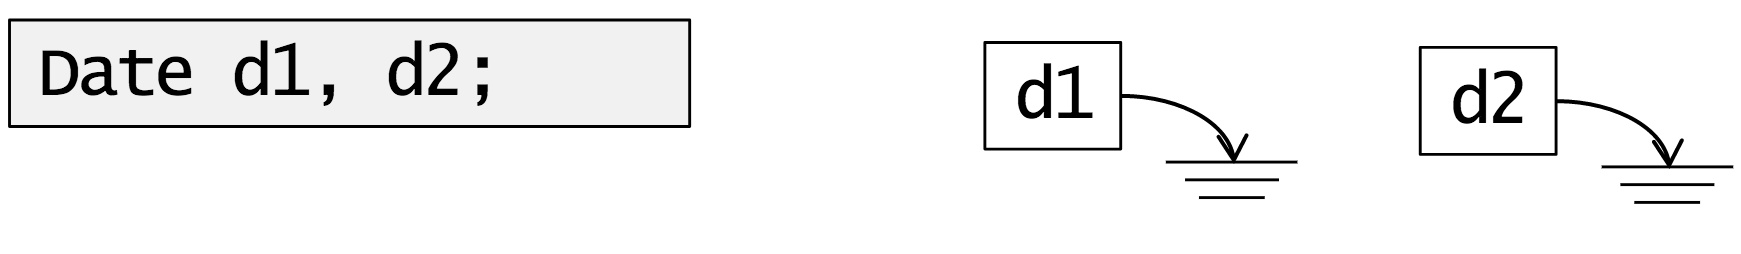
\includegraphics[width=.7\textwidth]{java/figures/basics/reference.png}
    \end{figure}
  \end{defn}
\end{defnbox}
\begin{notebox}[Note]\nospacing
  \begin{itemizenosep}
      \item Do not confuse C++ references with java references in Java variables are
  called (by convention) references.
      \item Reference variables are sort of C++ pointers but we can not do
    pointer arithmetic's on it e.g.\ \cppinline/ptr++/
      \item Reference Variables are of size:
    \begin{itemizenosep}
        \item 32-bit on a 32-bit JVM
        \item 32-bit of 64-bit on a 64-bit JVM, depending on the configuration
    \end{itemizenosep}
  \end{itemizenosep}
\end{notebox}
\begin{defnbox}\nospacing
  \begin{defn}[Static Type]\leavevmode
    A reference variable is declared to be of a specific type and that type,
    known as static type can never be changed.\leavevmode\\
    \ctr{Static type = type of reference variable}
  \end{defn}
\end{defnbox}
\begin{corbox}\nospacing
  \begin{cor}[Guarantees of Static Type]
    When a variable is declared as being of a particular type, then we have a
    language-enforced guarantee that any \textit{object} referenced by that
    reference variable will have (at least) all the features of that
    \textit{type}.\\
    $\Rightarrow$ \textit{dynamic type} needs to provide methods of \textit{static type}.
  \end{cor}  
\end{corbox}
\begin{defnbox}\nospacing
  \begin{defn}[Instanciation \javainline/new/]
    The new operator instantiates a class by dynamically allocating memory (=allocation at run time on the heap)
    for a new object and returns a reference to that memory.
    \begin{mintlinebox}{java}
      new MyClass();
    \end{mintlinebox}
    This reference can then be stored in/assigned to a (reference \cref{defn:referenceVariable}) variable.
    \begin{mintlinebox}{java}
      Type ref = new MyClass();
    \end{mintlinebox}
  \end{defn}
\end{defnbox}
\begin{notebox}[Note]\nospacing
  In Java, all class objects must be dynamically allocated.
\end{notebox}
%%% Local Variables:
%%% mode: latex
%%% TeX-master: "../../formulary"
%%% End:
